\documentclass{ctexart}
\usepackage{mathtools,amsfonts}
\usepackage{hyperref}
\usepackage{subcaption}
\usepackage{algorithm,algpseudocode}
\usepackage{listings}
\usepackage{mymacro}
\usepackage{biblatex}
\usepackage{color}

\definecolor{mygreen}{rgb}{0,0.6,0}
\definecolor{mygray}{rgb}{0.5,0.5,0.5}
\definecolor{mymauve}{rgb}{0.58,0,0.82}
\usepackage[a4paper,top=1in, bottom=1.25in, left=1.25in, right=1.25in]{geometry}
\graphicspath{{figures/}}
\addbibresource{ref.bib}
\title{深度学习初步及广告业务应用}
\author{张航}

\begin{document}
\lstset{
  language=Python,
 % basicstyle=\small
  basicstyle=\footnotesize\ttfamily,
  commentstyle=\color{mygreen},    % comment style
  escapeinside={\%*}{*)},          % if you want to add LaTeX within your
  keywordstyle=\color{blue},       % keyword style
  stringstyle=\color{mymauve},     % string literal style
} 

\maketitle
深度学习在人工智能领域有着广泛的应用,其在计算机视觉,自然语言处理等
方面取得了前所未有的成功。本文主要介绍一些最常用的神经网络结构,
并给出计算广告上面的可能应用。深度学习有诸多框架,包括Theano, Torch7,
MxNet和TensorFlow,它们各有特点, Bahrampour等\cite{bahrampour2015comparative}
对其性能做了比较. 本文介绍基于TensorFlow框架, 因为它通用性高, 更新快, 比较易用.

\section{深度学习的产生和分类}
神经网络起源于上世纪五、六十年代提出的感知器(perceptron)模型,
拥有输入层、输出层和一个隐含层, 输入的特征向量通过隐含层变换达到输出层。
之后随着数学和技术的发展,八十年代又提出了多层感知器(multilayer perceptron),
如\autoref{fig:mlp}所示. 若设第\(i\)个隐层的输入向量为\(h^{(i-1)}\),
输出向量为\(h^{(i)}\), 则
\[
  h^{(i)} = s(W^{(i)}h^{(i-1)}+b^{(i)}),
\]
其中\(W^{(i)},b^{(i)}\)是需要学习的权重矩阵和偏移向量, \(s(\cdot)\)为激活函数, 一般取sigmoid或者tanh函数,
\[
  \tanh(a)=\frac{e^a-e^{-a}}{e^a+e^{-a}},\quad \sigm(a)=\frac{1}{1+e^{-a}}.
\]
最后输出层一般用softmax函数变成分类器. 
多层感知在训练算法上使用反向传播(back propagation, BP)算法,
简单讲就是用梯度的链式法则计算每一层的梯度, 然后用SGD迭代优化.
\begin{figure}[htb]
  \centering
  \includegraphics[width=\textwidth]{mlp}
  \caption{上下层神经元全部相连的神经网络——多层感知器}
  \label{fig:mlp}
\end{figure}

显然感知器的层数越多,其刻画现实的能力就越强,不过要让神经网络变深并不容易。
首先随着层数增加,\emph{优化函数越来越容易陷入局部最优解}, 并且这个“陷阱”越来越偏离真正的全局最优。
数据量不大时训练出的深层网络,性能还不如较浅层网络。其次\emph{“梯度消失”现象更加严重},
以sigmoid激活函数为例, 对于幅度为1的信号, 在BP反向传播梯度时,每传递一层,梯度衰减为原来的0.20,
这样层数一多,梯度指数衰减后低层的梯度几乎为0,
找不到合适的迭代方向。最后\emph{深层网络将产生海量的参数},
对训练算法和计算机硬件都要求很高.

上述问题都很难解决,所以九十年代, 大家都转而研究浅层学习模型,
相继提出了支撑向量机(support vector machines, SVM)、
Boosting、最大熵方法(如Logistic Regression, LR)等.
这些模型的结构基本上可以看成带有一层隐层节点(如SVM、Boosting),
或没有隐层节点(如LR), 此时神经网络的研究相对沉寂.
不过卷积神经网络(CNN)是个特例, 它在层数增多的时候相对容易训练且效果很好,
所以在1998年提出后, 很快就被美国银行业用于支票等单据的手写数字识别.
CNN易于训练的性质还没有在理论上找到明确的原因.

2006年,加拿大多伦多大学教授、机器学习领域泰斗Geoffrey Hinton和
他的学生Ruslan Salakhutdinov在《科学》上发表了一篇文章\cite{hinton2006reducing},
开启了神经网络在学术界和工业界的新纪元.
他们利用预训练方法缓解了局部最优解问题, 将隐层数提升到了7.
所谓预训练就是在做有监督学习之前先做无监督学习, 用无监督学习出一些优异的
初始参数后再做有监督学习调优, 这样可以得到更好的效果.
Hinton使用了逐层优化的多层限制玻尔兹曼机(Restricted Boltzmann machine, RBM),
又称作Deep Belif Network(DBN). 之后Bengio等\cite{bengio2007greedy}提出了
Deep autoencoder模型也可以做无监督的特征学习.

后来的LSTM模型在RNN上解决了梯度消失的问题, 常常用于时序模型.而海量参数
的问题被大规模训练数据, 并行GPU运算和各种正则化技巧、优化技巧解决.

\section{卷积神经网络(CNN)}
1998年LeCun等\cite{lecun1998gradient}将CNN运用于手写数字识别, 取得了巨大
的成功, 下面结合手写数字数据集MINIST介绍CNN. \autoref{fig:cnn}
是一个典型的CNN网络, 它包括两个卷积层和一个全连接层.
\begin{figure}[htb]
  \centering
  \includegraphics[width=.9\textwidth]{Typical_cnn}
  \caption{CNN结构}
  \label{fig:cnn}
\end{figure}

MNIST是一个入门级的计算机视觉数据集,它包含各种手写数字图片\\
{\centering
  \includegraphics[width=.7\textwidth]{minist}\\
}
它也包含每一张图片对应的标签,告诉我们这个是数字几。
比如,上面这四张图片的标签分别是5,0,4,1。
我们要训练一个机器学习模型用于预测图片里面的数字.

\subsection{卷积}

首先介绍卷积, 直接给出一个具体的例子:假设你已经有
一个3x3的卷积核, 那么就可以用它提取5x5的样本所具有的特征.
如\autoref{fig:conv}所示, 我们对5x5的图像的每个3x3 的小块
图像区域都进行卷积运算, 结果变为3x3个卷积特征.
\begin{figure}[htb]
  \centering
  \includegraphics[width=.8\textwidth]{conv}
  \caption{对每个小块做卷积}
  \label{fig:conv}
\end{figure}

对于一个复杂的图片, 一种卷积核能提取的特征很有限, 需要
结合多种卷积核. CNN一个不同于以往方法之处就是没有人为
指定卷积核, 而是通过数据学习出来. CNN的一个卷积层如\autoref{fig:convlayer}
所示. 我们指定卷积核的个数\(k\), 然后作用于上一层的每一输入图片,
这样下一层的图片就更上一层的\(k\)倍.
\begin{figure}[htb]
  \centering
  \includegraphics[width=.7\textwidth]{convlayer}
  \caption{CNN的一个卷积层}
  \label{fig:convlayer}
\end{figure}

\subsection{池化}
CNN的另一个重要概念是池化(Max-pooling).
它可以降采样, 加快运算速度, 又提供了某种
平移不变性. 池化很简单, 如2x2池化如\autoref{fig:maxpool}所示,
将4x4的图片降到2x2.
\begin{figure}[htb]
  \centering
  \includegraphics[width=.8\textwidth]{Max_pooling}
  \caption{最大池化}
  \label{fig:maxpool}
\end{figure}

\subsection{TensorFLow实现}
TensorFlow提供了卷积和池化的函数, 如果把每一层的输入\(x\)
看作一个4维矩阵(由于可能有RGB信息, 图片是三维矩阵,那么多张
图片就是4维), 即一个张量(tensor), 并且卷积核参数\(W\)
也是一个4维张量. 我们使用下面的函数计算卷积和池化.
\begin{lstlisting}
import tensorflow as tf
def conv2d(x, W):
  return tf.nn.conv2d(x, W, strides=[1, 1, 1, 1], padding='SAME')

def max_pool_2x2(x):
  return tf.nn.max_pool(x, ksize=[1, 2, 2, 1],
                        strides=[1, 2, 2, 1], padding='SAME')
\end{lstlisting}

由于MINIST的输入图片是\(28\times28\)的灰度图片, 所以初始化为
\(n\times28\times28\times1\)的张量. 设卷积在每个5x5的patch中算出32个特征
于是\(w\)是\(5\times5\times1\times32\).
\begin{lstlisting}
x_image = tf.reshape(x, [-1,28,28,1])
# 初始化第一个隐层的参数
W_conv1 = weight_variable([5, 5, 1, 32])
b_conv1 = bias_variable([32])
# 计算第一个隐层
h_conv1 = tf.nn.relu(conv2d(x_image, W_conv1) + b_conv1)
h_pool1 = max_pool_2x2(h_conv1)
\end{lstlisting}
第二个隐层类似, 只是取了64个特征. 经过两次池化,
图片尺寸减小到7x7,我们加入一个有1024个神经元的全连接层, 然后用
Softmax分类器即可. 这里还有一个防止过拟合的技巧:Dropout, 因为
全连接层有1024个神经元, 数量较多, 可以在每次训练时随机舍弃一些
神经元, 即dropout. 训练和预测代码如下, CNN在测试集上的准确率达到
了99.2\%.
\begin{lstlisting}
cross_entropy = -tf.reduce_sum(y_*tf.log(y_conv))
train_step = tf.train.AdamOptimizer(1e-4).minimize(cross_entropy)
correct_prediction = tf.equal(tf.argmax(y_conv,1), tf.argmax(y_,1))
accuracy = tf.reduce_mean(tf.cast(correct_prediction, "float"))
sess.run(tf.initialize_all_variables())
for i in range(20000):
  batch = mnist.train.next_batch(50)
  if i%100 == 0:
    train_accuracy = accuracy.eval(feed_dict={
        x:batch[0], y_: batch[1], keep_prob: 1.0})
    print "step %d, training accuracy %g"%(i, train_accuracy)
  train_step.run(feed_dict={x: batch[0], y_: batch[1], keep_prob: 0.5})

print "test accuracy %g"%accuracy.eval(feed_dict={
    x: mnist.test.images, y_: mnist.test.labels, keep_prob: 1.0})
\end{lstlisting}

\section{RBM和DAE}
下面介绍Hinton在2006年提出的deep belief network(DBN). Hinton用DBN做
无监督学习的特征提取, 使用DBN后再用LR, SVM等分类器通常可以得到更好的
结果. DBN是逐层优化的限制玻尔兹曼机(RBM), 所以下面先介绍RBM.
\subsection{RBM}
RBM的想法是我们观测到的特征是有一些无法观测到的隐层特征决定的,
假定隐层变量互相独立, 且满足某种特定分布(一般取0-1的二项分布),
那么我们可以用这种结构, 模拟任何一种分布, 并通过极大似然估计的
方法确定出模型参数. 这样我们得到的隐层特征就是更本质的特征.
\begin{figure}[htb]
  \centering
  \includegraphics[width=.8\textwidth]{rbm}
  \caption{RBM是一个二部图: v是观测, h是隐层}
  \label{fig:rbm}
\end{figure}

\autoref{fig:rbm}的能量函数\(E(v,h)\)定义为:
\[
  E(v,h) = - b^Tv - c^Th - h^TWv
\]
一般情况下假设 \(v_j, h_i \in \{0,1\}\), 那么
可以推出下面两个条件概率:
\begin{align*}
  \P(h_i=1|v)& = \sigm(c_i + W_i v), \\
  \P(v_j=1|h)& = \sigm(b_j + W'_j h).
\end{align*}
下一步要得出参数的梯度, 这里需要用到Gibbs采样和Hinton提出的Contrastive
Divergence算法.
RBM模型具体的理论推导以及算法可以参考\cite{fischer2012introduction}.

RBM的TensorFlow实现也相对比较复杂, 不过
\url{http://deep-learning-tensorflow.readthedocs.io/en/stable/}
给出了包括RBM在内的很多模型的开源实现.
RBM是深度学习中很重要的基础结构, 被大量用于各种模型中, 也有多种变形
比如convolutional RBM\cite{lee2009convolutional}, temporal
RBM\cite{sutskever2009recurrent}等.

\begin{figure}[t]
  \centering
  \includegraphics[width=.7\textwidth]{autoencoder}
  \caption{Autoencoder}
  \label{fig:autoencoder}
\end{figure}
\subsection{DAE}
继DBN后, Bengio等\cite{bengio2007greedy}提出了一种类似的
特征提取深度网络: deep autoencoder(DAE). 它也是一种逐层优化的结构, 其中
最基础的一层如\autoref{fig:autoencoder}所示. 如果原始输入
是6维, 隐层是3个节点, 输出也是6个. 输入到隐层是encode, 隐层
到输出是decode.

最简单的情形, autoencoder将\( \mathbf{x} \in \mathbb{R}^d\)
映射到\(\mathbf{h} \in \mathbb{R}^p\)
\[
  \mathbf{h} = s_1(\mathbf{Wx}+\mathbf{b})
\]
然后我们再从\(\mathbf{h}\)中重建\(\mathbf{x}\)
\[
  \mathbf{x'} = s_2(\mathbf{W'h}+\mathbf{b'})
\]
Autoencoder的目标就是极小化重建误差:
\[
  \mathcal{L}(\mathbf{x},\mathbf{x'})=
  \|\mathbf{x}-\mathbf{x'}\|^2=
  \|\mathbf{x}-s_2(\mathbf{W'}(s_1(\mathbf{Wx}+\mathbf{b}))+\mathbf{b'})\|^2
\]
对于一次优化后的结果, 我们可以去掉\(W', b'\), 继续将\(\mathbf{h}\)作为
下一层的输入优化新的一层. DAE相对DBN计算量小, 在应用中它们
的表现互有胜负, \cite{cho2013boltzmann,deng2010binary}在图片识别和语音识别
领域对它们做了比较.

%\section{LSTM和RNN}
%未完成

\section{广告应用}
深度学习在很多方面取得的巨大成功, 比如图片识别领域, 现在ImageNet上识别率较高的
模型几乎没有不采用神经网络的. 不过在广告领域还没有看到公认的巨大成果, 百度宣称使用
DNN模型使得点击率预估性能提升了20\%, 但是没有说明比较的基准是
线性的LR模型, 还是非线性的GBDT+FM.
目前也没有公司公开的自己用于广告的深度学习模型, 不过还是有些学术上的研究成果.
Zhang等\cite{zhang2016deep}提出了基于FM的Factorization-machine supported Neural
Network(FNN)和基于RBM, DAE的Sampling-based Neural Network(SNN)两种模型改进CTR估计.

首先假设输入数据的每一特征都是离散的, 比如对于城市这个特征,
每个样本只能从北京、上海、广州、深圳选项中选其一, 这样输入特征向量\(\bs{x}\)在每个
类别上是一个one-hot向量. 下面介绍两种神经网络结构.

\subsection{FNN}

\begin{figure}[htb]
  \centering
  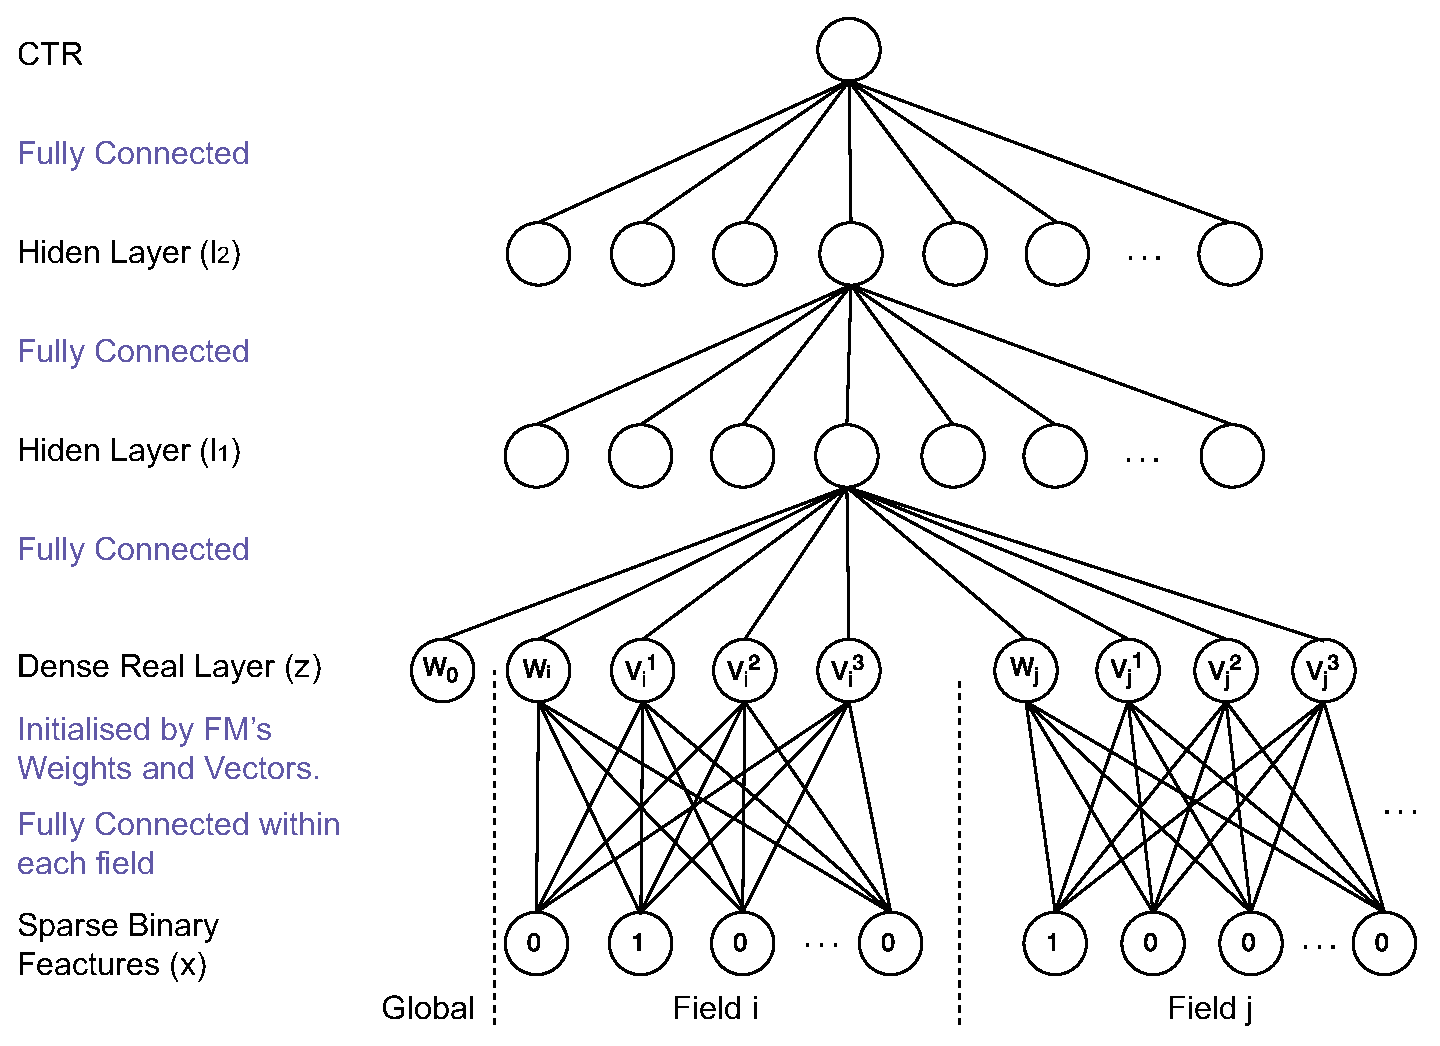
\includegraphics[width=0.75\columnwidth]{dlctr}
  \caption{ 4层的FNN结构}\label{fig:modelone}
\end{figure}

FNN在最下面一层基于factorisation machine(FM)\cite{rendle2012factorization},
整个结构如\autoref{fig:modelone}所示.
从上到下看, 最上面的输出层是一个实数\(\hat{y} \in (0,1)\)即预估的CTR:
\begin{equation}
  \hat{y} =\sigm(\bs{W}_{3}\bs{l}_{2}+b_{3}),   \label{eq:xdef1}
\end{equation}
其中 $\bs{W}_{3}\in\mathbb{R}^{1 \times L}$, $b_{3}\in \mathbb{R}$ 且 $\bs{l}_{2} \in \mathbb{R}^{L}$
是这一层的输入. $\bs{l}_{2}$来自
\begin{equation}
  \bs{l}_{2}=\tanhh(\bs{W}_{2}\bs{l}_{1}+\bs{b}_{2}),   \label{eq:xdef2}
\end{equation}
其中$\bs{W}_{2}\in\mathbb{R}^{L\times M}$, $\bs{b}_{2}\in \mathbb{R}^{L}$ 且 $\bs{l}_{1} \in \mathbb{R}^{M}$.
作者对激活函数 $\tanh(\cdot)$ 的选择做了一些讨论. 下一层类似
\begin{equation}
  \bs{l}_{1}=\tanhh(\bs{W}_{1}\bs{z}+\bs{b}_{1}),   \label{eq:xdef3}
\end{equation}
其中 $\bs{W}_{1}\in\mathbb{R}^{M\times J}$, $\bs{b}_{1}\in \mathbb{R}^{M}$ 和 $\bs{z} \in \mathbb{R}^{J}$.
\begin{equation}
  \bs{z}=(w_{0}, \bs{z}_{1}, \bs{z}_{2}, ...\bs{z}_{i}, ..., \bs{z}_{n}),
  \label{eq:xdef4}
\end{equation}
其中 $w_{0} \in \mathbb{R}$ 是全局缩放参数, $n$是类别个数.
$\bs{z}_{i} \in\mathbb{R}^{K+1}$ 来自factorisation machines:
\begin{equation}
  \bs{z}_{i}=\bs{W}_{0}^{i}\cdot \bs{x}[\tstart_{i}:\tend_{i}] = (w_i, v_i^1, v_i^2, \ldots, v_i^K),
  \label{eq:xdef5}
\end{equation}
其中 $\tstart_{i}$ 和 $\tend_{i}$是第$i$类的特征编号开始和结束位置,
$\bs{W}_{0}^{i} \in \mathbb{R}^{(K+1) \times (\tend_{i}-\tstart_{i}+1)} $
的每一列都是来自FM训练出得参数, FM模型如下
\begin{equation}
   y_{\text{FM}}(\bs{x}):=\sigm \left( w_{0}+\sum_{i=1}^{N} w_{i} x_{i}
   +\sum_{i=1}^{N}\sum_{j=i+1}^{N}\langle\bs{v}_{i},\bs{v}_{j}\rangle x_{i}
   x_{j} \right).
   \label{eq:xdef}
\end{equation}
用FM训练出得每个特征因子向量和bias初始化参数矩阵\(\bs{W}_{0}^i\), 其它隐层
参数是用逐层优化的RBM进行初始化\cite{bengio2007greedy},
然后在是使用实际数据的0-1标签做supervised fine-tuning,
损失函数用cross entropy
\begin{equation}
  L(y,\hat{y})= -y\log \hat{y} - (2-y)\log(1-\hat{y}), \label{eq:xdefloss}
\end{equation}
使用back propagation更新参数.

\begin{figure}[tb]
  \centering
  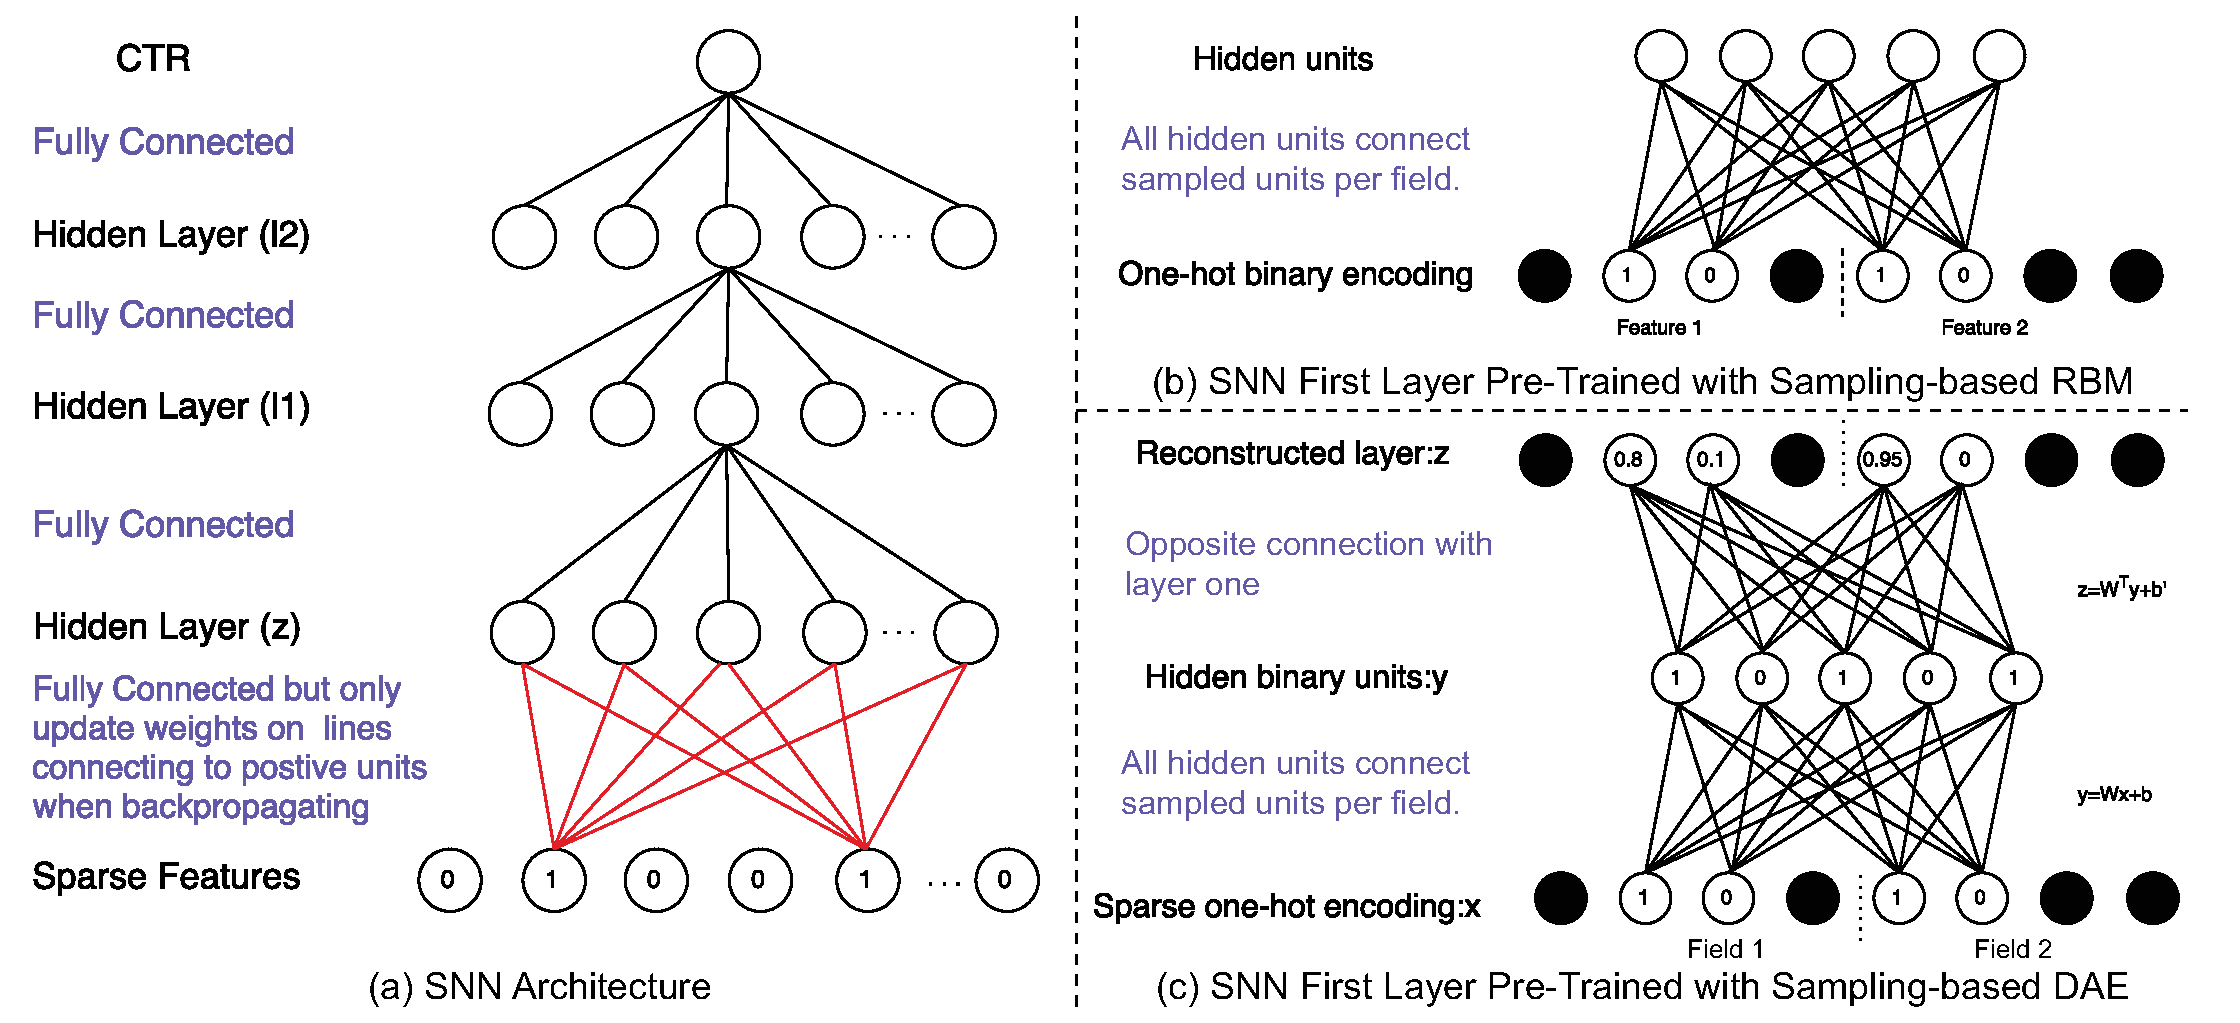
\includegraphics[width=1.1\columnwidth]{ssn3}
  \caption{4层的SNN结构以及两种pre-training方法.}\label{fig:snn}
\end{figure}
\subsection{SNN}
SNN和FNN类似, 只是最底下一层是全连接的, 并且不通过FM而是用RBM或DAE初始化参数.
如\autoref{fig:snn}(a)所示, SNN最底下一层为:
\begin{equation}
  \bs{z}=\sigmoid(\bs{W}_{0}\bs{x}+\bs{b}_{0}).   \label{eq:defmodtwo}
\end{equation}
参数的初始化使用RBM或者DAE. 为了降低高维稀疏one-hot数据的计算复杂度, 作者提出
了sampling-based RBM\autoref{fig:snn}(b)和sampling-based DAE\autoref{fig:snn}(c).

为了降低计算成本, 对每个样本某个特征类只取一个正单元和\(m\)个负单元, 比如对于
某个样本, city这个特征字段是北京, 那么它对应的one-hot向量是\((1, 0, 0, 0)\),
这是我们取\(m=1\), 从剩下三个城市中随机采样一个, 比如取了上海, 那么没有采样
到的特征对应的参数就不用更新了, 这是的one-hot向量就是\((1, 0)\), 维数将为
\(m+1\). RBM做constrastive divergence(\autoref{alg:sampleRBM})
和DAE做SGD时, 需要更新的参数数量大大减少.

\begin{algorithm}[t]
  \caption{Algorithm for getting initial weights via sampled CD-1}
  \label{alg:sampleRBM}
  \begin{algorithmic}
  \renewcommand{\algorithmicrequire}{\textbf{Input:}}
  \renewcommand{\algorithmicensure}{\textbf{Output:}}
    \Require sample number $k$, input vector $x$, feature number $n$, learning rate $\lambda$
    \Ensure gradient approximation $W $ and $ b$
\For  {all feature units}
    \State 	   $ sx \leftarrow $ sample $x_{i}$ if its value is one.
         \For  {1 to k-1}
              \State   $sx  \leftarrow $ sample $x_{i}$ if the value $x_{i}$ is zero.
         \EndFor
    \EndFor
    \State  $sW$, $sb \leftarrow W$, $b$
    \Statex\Comment{\%comment: only assign from $W/b$ according to the sampled indexes\%}
    \State $x_{2}$, $h_{1}$, $h_{2}$=Gibbs($sx$, $sW$, $sb$)
    \State  $ sW \leftarrow $  $sW+\lambda(h_{1}\cdot sx-h_{2}\cdot x_{2})   $
    \State $ sb \leftarrow $  $sb + \lambda(sx-x_{2})$
    \State $ c \leftarrow  $   $c +\lambda(h_{1}-h_{2})$
    \State $ W $, $b \leftarrow sW$, $sb$
	\Statex\Comment{\%comment: only assign into $W/b$ according to the sampled indexes\%}
  \end{algorithmic}
\end{algorithm}
\subsection{效果}
\begin{table}[t]
\centering
\caption{不同模型CTR预估的AUC表现.}\label{tab:performance}
\begin{tabular}{c|ccccc}
& ~~~~LR~~~~ & ~~~~FM~~~~ & ~~~FNN~~~ & SNN-DAE & SNN-RBM\\ \hline
1458 & 70.42\% & 70.21\% & \textbf{70.52\%} & 70.46\% & 70.49\% \\
2259 & 69.66\% & 69.73\% & \textbf{69.74\%} & 68.08\% & 68.34\% \\
2261 & 62.03\% & 60.97\% & 62.99\% & \textbf{63.72\%} & \textbf{63.72\%} \\
2997 & 60.77\% & 60.87\% & 61.41\% & \textbf{61.58\%} & 61.45\% \\
3386 & 80.30\% & 79.05\% & \textbf{80.56\%} & 79.62\% & 80.07\% \\
all  & 68.81\% & 68.18\% & \textbf{70.70\%} & 69.15\% & 69.15\% \\
\end{tabular}
\end{table}

作者在iPinYou\cite{liao2014ipinyou}数据上做了测试, 数据集中包括1950万样本,
1.479万正样本, 01化之后的特征维度是93.767万. \autoref{tab:performance}
展示了不同算法在5个不同广告主和整个样本上的AUC表现, 可以看出新算法有不小的提升.
文章中还有很多细节, 包括正则化, 超参数调优, 结构调整等等, 这里不展开介绍.

\subsection{其它应用}
深度学习还能从非结构话的数据中提取特征,
比如Fire等\cite{fire2015exploring} 使用CNN从图片类型的
广告中提取信息, 提高了CTR预估准确率. 使用LSTM处理
广告和曝光中的文本信息也是一种思路.

\printbibliography

\end{document}

